\documentclass[a4paper, 12pt]{article}

\usepackage[italian]{babel}
\usepackage{tikz}
\usepackage{xcolor}
\usepackage{graphicx}
\usepackage{hyperref}
\usepackage{imakeidx}
\usepackage{caption}
\usepackage{fancyhdr}
\usepackage{geometry}
\usepackage{tabularx}


%--------------------VARIABILI--------------------
\def\logo{../Immagini/logo.jpeg}
\def\ultima-versione{v0.1}
\def\titolo{Piano di Progetto}
%------------------------------------------------

\usetikzlibrary{calc}
\definecolor{fp-blue}{HTML}{2885c8}
\definecolor{fp-red}{HTML}{ea5f64}
\makeindex[title=Indice]
\hypersetup{
    hidelinks,
    colorlinks=true,
    linkcolor=fp-red,
    filecolor=magenta,      
    urlcolor=fp-blue,
    pdfpagemode=FullScreen,
}

\pagestyle{fancy}
\fancyhead[L]{}
\setlength{\headheight}{15pt}
\fancyhead[R]{\titolo \space - \ultima-versione}

\renewcommand{\familydefault}{\sfdefault}
\newcommand{\glossario}[1]{\fontfamily{lmr}\selectfont{\textit{#1\textsubscript{\small G}}}}
\newcolumntype{C}{>{\centering\arraybackslash}X}

%--------------------INFORMAZIONI PRIMA PAGINA-------------------- 
\title{\Huge \textbf{\titolo}}
\author{\Large{Alt} \raisebox{0.3ex}{\normalsize  +} \Large{F4}}
\date{19 Novembre 2024}
%----------------------------------------------------------------

\begin{document}

\begin{titlepage}      
    \maketitle
    \thispagestyle{empty}  

    \begin{tikzpicture}[remember picture, overlay]
        \fill[fp-blue] 
        ($(current page.south west) + (0, 10)$) 
        -- ($(current page.center) + (0, -8)$)
        -- ($(current page.center) + (0, -15)$)
        -- (current page.south west);

        \fill[fp-red]
        ($(current page.south east) + (0, 10)$) 
        -- ($(current page.center) + (0, -8)$)
        -- ($(current page.center) + (0, -15)$)
        -- (current page.south east);

        \clip ($(current page.center) + (0, -8)$) circle (1cm) node 
        {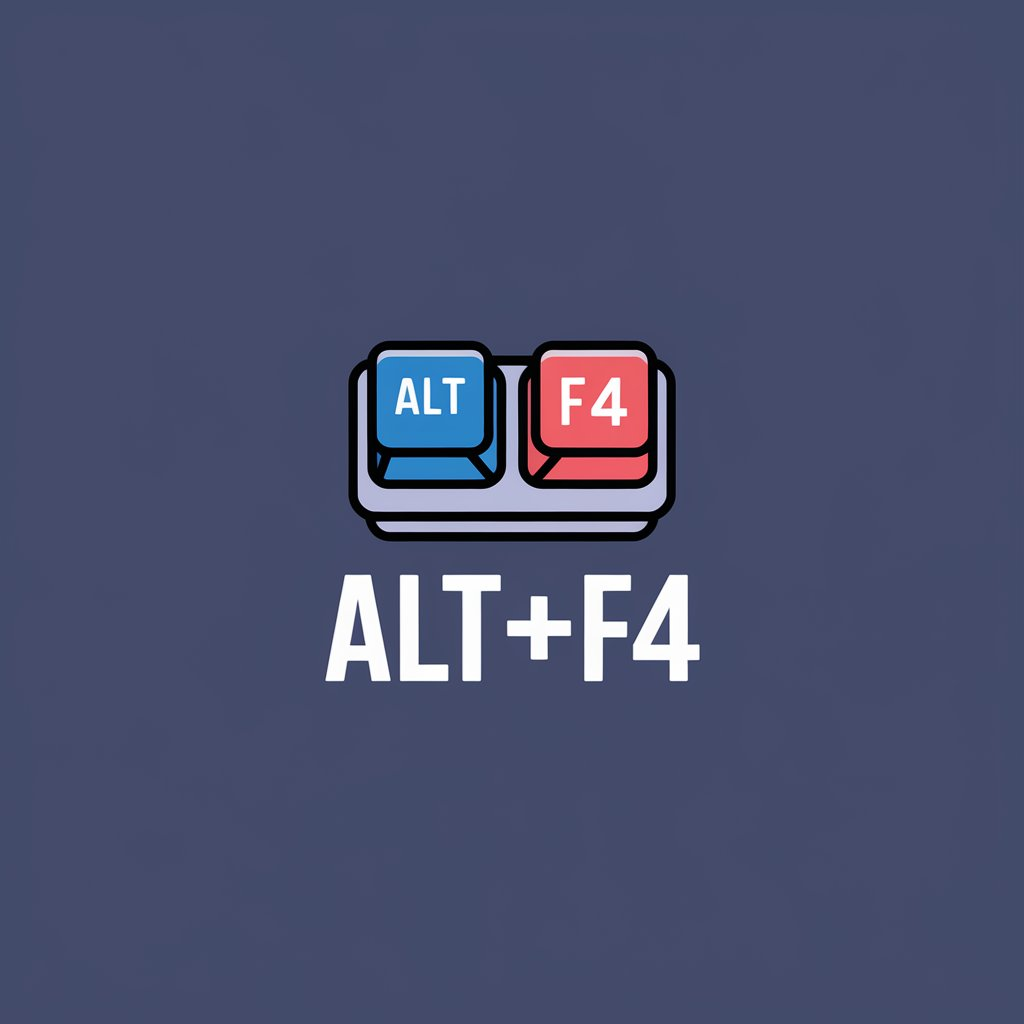
\includegraphics[width=.25\textwidth]{\logo}};
        
    \end{tikzpicture}    
\end{titlepage}

\thispagestyle{plain}
\newgeometry{ignoreall, hmargin=20pt}
\begin{table}[!h]
    \centering
    \caption*{\textbf{\Large Registro Modifiche}}
    {\renewcommand{\arraystretch}{2}
    \begin{tabularx}{\textwidth}{| c | c | C | C | C |}
        \hline
            \textbf{\normalsize Versione} & 
            \textbf{\normalsize Data} & 
            \textbf{\normalsize Autore/i} & 
            \textbf{\normalsize Verificatore} &
            \textbf{\normalsize Descrizione} \\ 
        \hline \hline
        v0.1 & 
        19 novembre 2024  & 
        Enrico Bianchi &
        Francesco Savio& 
        Sottosezioni \hyperref[sec:intro]{Introduzione documento}, \hyperref[sec:adr]{Analisi dei rischi} \\
        \hline 
    \end{tabularx}}
\end{table}
\restoregeometry

\tableofcontents

\newpage

\section{Introduzione}
\label{sec:intro}
Questo documento ha lo scopo di fornire informazioni dettagliate su come il progetto verrà gestito dal team.
Nello specifico gli argomenti trattati saranno:
\begin{itemize}
    \item \textbf{analisi dei rischi}
    \item \textbf{suddivisione dei ruoli}
    \item \textbf{modello di sviluppo adottato}
    \item \textbf{stima dei costi}
\end{itemize}

\section{Analisi dei rischi}
\label{sec:adr}
L'analisi dei rischi è una fase cruciale nella gestione di un progetto software in quanto consente di identificare, valutare e mitigare
i vari problemi che potrebbero compromettere la buona riuscita del progetto. Lo scopo di questa attività è quindi prevedere eventi indesiderati
che potrebbero influenzare negativamente i tempi, i costi e la qualità del prodotto finale.
Il processo di gestione dei rischi è suddiviso in quattro fasi:
\begin{enumerate}
    \item \textbf{identificazione}, innanzitutto è necessario identificare il maggior numero di fattori di rischio per il progetto.
    \item \textbf{analisi}, durante la quale si studiano le probabilità di occorrenza dei rischi e le conseguenze nel caso dovessero verificarsi.
    \item \textbf{pianificazione}, fase in cui si analizza come evitare i rischi e come mitigarne gli effetti 
    \item \textbf{controllo}, ultima fase durante la quale si può successivamente ritornare alla fase di analisi, durante questa fase vi è una continua verifica di rilevazioni di rischi e 
    l'attuazione delle strategie di mitigazione. 
\end{enumerate}
I rischi individuati verranno descritti nel seguente modo:
\begin{itemize}
    \item \textbf{tipologia}: cioè la categoria a cui appartiene il rischio, può essere organizzativa o tecnologica.
    \item \textbf{indice}: indice numerico che identifica un rischio per ogni tipologia.
    \item \textbf{descrizione}: descrizione dl rischio.
    \item \textbf{pericolosità}: può essere bassa, media o alta e indica l'impatto che avrebbe sul progetto il suo verificarsi.
    \item \textbf{probabilità}: può essere bassa, media o alta e indica la probabilità del rischio di verificarsi.
    \item \textbf{prevenzione}: indica la metodologia utilizzare per identificare il rischio.
    \item \textbf{mitigazione}: azioni da intraprendere quando si verifica il rischio.   
\end{itemize}
Ogni rischio verrà indicato con la sigla R[tipologia][identificativo].
\subsection{Rischi organizzativi}
\subsubsection{RO1: Impegni universitari}
\begin{itemize}
    \item \textbf{Descrizione}: la preparazione per esami universitari può diminuire la disponibilità di uno o più membri del gruppo.
    \item \textbf{Pericolosità}: Media
    \item \textbf{Probabilità}: Alta
    \item \textbf{prevenzione}: è importante condividere le date in cui si verranno svolti gli esami e in cui, essendo più impegnati 
    con lo studio individuale, si pensa di poter dare meno disponibilità per il progetto.
    \item \textbf{Mitigazione}: sarà compito del responsabile gestire il carico di lavoro e le attività da svolgere, basandosi sulle ore disponibili per ogni membro,
    in modo tale da garantire il rispetto delle scadenze. In casi gravi il responsabile dovrà occuparsi della modifica delle risorse per lo sprint
    o della scadenza.
\end{itemize}
\subsubsection{RO2: Impegni personali}
\begin{itemize}
    \item \textbf{Descrizione}: un membro potrebbe garantire una minore disponibilità durante un periodo a causa di impegni di natura personale.
    \item \textbf{Pericolosità}: Bassa
    \item \textbf{Probabilità}: Media
    \item \textbf{prevenzione}: importante avvisare tempestivamente e con il maggior anticipo possibile i giorni in cui non si sarà disponibili. 
    \item \textbf{Mitigazione}: è compito del responsabile calcolare le ore disponibili del gruppo durante lo sprint e organizzare il carico di lavoro tenendo conto di 
    tutti gli impegni precedentemente comunicati dai compagni. 
\end{itemize}
\subsubsection{RO3: Errori di pianificazione delle attività}
\begin{itemize}
    \item \textbf{Descrizione}: l'inesperienza dei membri del gruppo nel contesto della pianificazione di progetto è un fattore di rischio rilevante
    che può interferire sulla corretta realizzazione del progetto. Nello specifico, la mancata esperienza nell'ambito può portare a una sottostima 
    delle risorse necessarie allo sviluppo delle attività o a un errata valutazione delle tempistiche. 
    \item \textbf{Pericolosità}: Alta
    \item \textbf{Probabilità}: Alta
    \item \textbf{prevenzione}: continuo controllo del Piano di Progetto per monitorare le risorse utilizzate e il tempo in cui sono state impiegate.
    Aggiornamento tra i membri del gruppo tramite Telegram sul proseguo nello sviluppo delle attività.
    \item \textbf{Mitigazione}: in caso dovessero verificarsi difficoltà o ritardi è compito del responsabile rivedere il Piano di Progetto e 
    modificare il numero delle risorse allocate per lo sprint o, in casi gravi, la scadenza.
\end{itemize}
\subsubsection{RO4: Scarsa collaborazione di uno o più membri del gruppo}
\begin{itemize}
    \item \textbf{Descrizione}: rischio dovuto alla possibilità che uno o più membri impieghino scarso impegno nella realizzazione del progetto.
    \item \textbf{Pericolosità}: Alta
    \item \textbf{Probabilità}: Bassa
    \item \textbf{prevenzione}: è stata da subito richiesta la massima trasparenza tra i membri del gruppo.
    Sarà compito del responsabile verificare che ogni membro abbia partecipato equamente nella realizzazione delle attività dello sprint.
    \item \textbf{Mitigazione}: Il responsabile dovrà contattare e avvisare il membro che, senza preavviso, non avrà impiegato le giuste risorse personali nello sviluppo delle attività dello sprint,
    in modo tale da chiarire eventuali complicanze o fraintendimenti. 
\end{itemize}
\subsubsection{RO5: Disaccordi all'interno del gruppo}
\begin{itemize}
    \item \textbf{Descrizione}: possono generarsi discussioni a causa di opinioni e ideologie diverse all'interno del gruppo.
    \item \textbf{Pericolosità}: Alta
    \item \textbf{Probabilità}: Media
    \item \textbf{prevenzione}: importante che vi sia chiarezza e trasparenza durante le chiamate del gruppo, bisogna dichiarare da subito
    eventuali discordanze su idee e opinioni in modo da trovare un punto d'incontro più rapidamente possibile.
    \item \textbf{Mitigazione}: in caso in cui non si riesca a raggiungere un compromesso definitivo le varie opzioni su cui si sta discutendo verranno messe a votazione, verrà scelta l'opzione, o le opzioni, che hanno la maggioranza dei voti. 
\end{itemize}
\subsubsection{RO6: Risorse disponibili ma non impiegate}
\begin{itemize}
    \item \textbf{Descrizione}: ruoli come amministratore, progettista o verificatore passeranno dei periodi in cui avranno un carico 
    di lavoro e uno sforzo produttivo inferiore ad altri ruoli. Se quindi uno o più membri del gruppo focalizzeranno il proprio lavoro solo
    su uno di questi ruoli potrebbero non impiegare tutte le loro ore produttive disponibili durante lo sprint.
    \item \textbf{Pericolosità}: Alta
    \item \textbf{Probabilità}: Bassa
    \item \textbf{prevenzione}: viene creata una tabella per la rendicontazione delle ore per ogni sprint nel piano di progetto che ogni membro dovrà compilare.
    Il responsabile potrà quindi, attraverso la tabella, verificare le attività e le ore impiegate per ogni ruolo in modo tale da rilevare se c'è una disponibilità di risorse non sfruttate.
    \item \textbf{Mitigazione}:  Per ogni sprint viene creata una dashboard su GitHub con tutte le attività da svolgere durante lo sprint.
    Ogni membro potrà assegnarsi attività da svolgere anche di ruoli diversi in modo tale che ognuno impieghi nel modo piè efficiente possibile le proprie ore produttive.
\end{itemize}

\subsection{Rischi tecnologici}
\subsubsection{RT1: Inesperienza sulle tecnologie da adottare}
\begin{itemize}
    \item \textbf{Descrizione}: La mancata competenza di alcuni o tutti i membri del gruppo nell'utilizzo di tecnologie utili alla realizzazione del progetto,
    come le tecnologie di verifica di attendibilità di una risposta data da un modello LLM, potrebbero causare rallentamenti nello sviluppo, con particolare
    attenzione alle fasi di progettazione, verifica e progettazione. 
    \item \textbf{Pericolosità}: Alta
    \item \textbf{Probabilità}: Alta
    \item \textbf{prevenzione}: All'inizio di ogni sprint è necessario che, a fronte delle attività che si dovranno svolgere, ogni membro 
    del gruppo esponga eventuali dubbi per quanto riguarda l'utilizzo di tecnologie adottate. Sarà inoltre compito del responsabile controllare
    alla fine di ogni sprint le ore assegnate inizialmente e poi quelle realmente impiegate per svolgere ogni attività, in modo da comprendere
    quali tecnologie hanno causato rallentamenti durante lo svolgimento.
    \item \textbf{Mitigazione}:  Innanzitutto ogni membro garantisce impegno individuale nello studio delle tecnologie necessarie.
    È stato realizzato un documento condiviso su cui ogni membro andrà ad aggiungere una descrizione degli argomenti appresi durante lo studio 
    individuale in modo che tutto il gruppo rimanga aggiornato sulle tecnologie che potrebbero essere adottate nello sviluppo del progetto.
    È stata creata una chat Discord in cui verranno condivisi articoli e documenti inerenti alle tecnologie studiate.
    Ogni membro del gruppo è inoltre disponibile per chiarimenti e supporto per quanto riguardano le tecnologie in cui possiede maggiore esperienza.
\end{itemize}
\subsubsection{RT2: Malfunzionamenti hardware}
\begin{itemize}
    \item \textbf{Descrizione}: Eventuali guasti e anomalie ai componenti hardware utilizzati dai membri del gruppo potrebbero causare 
    interruzioni nello sviluppo del progetto con la possibilità di ritardi nella consegna.
    \item \textbf{Pericolosità}: Alta
    \item \textbf{Probabilità}: Bassa
    \item \textbf{prevenzione}: È necessaria una segnalazione immediata a tutti i membri del gruppo in caso di un guasto al proprio sistema.
    \item \textbf{Mitigazione}: Nel caso in cui un membro non fosse disponibile per via di guasti hardware il responsabile deve 
    rivalutare il Piano di Progetto e rivedere le risorse disponibili per lo sprint in base alla disponibilità degli altri membri.
    È inoltre essenziale lavorare maggiormente possibile in un ambiente condiviso per ridurre la perdita di informazioni.
\end{itemize}
\subsubsection{RT3: Inadeguata conoscenza degli strumenti di sviluppo software}
\begin{itemize}
    \item \textbf{Descrizione}: Alcuni membri del gruppo potrebbero avere competenze ridotte nell'utilizzo di software di terze parti necessari allo sviluppo, 
    come sistemi di versionamento del codice, di automazione della build o di containerizzazione. 
    \item \textbf{Pericolosità}: Alta
    \item \textbf{Probabilità}: Alta
    \item \textbf{prevenzione}: Ogni membro del gruppo deve verificare la sua capacità di utilizzo degli strumenti adottati e segnalare ai compagni
    eventuali dubbi.
    \item \textbf{Mitigazione}: Sarà compito dell'amministratore aggiornare continuamente le Norme di Progetto con una descrizione esaustiva
    e comprensibile a tutti i membri degli strumenti adottati, dei loro casi d'uso e di eventuali comandi da terminale necessari per il progetto.
\end{itemize}
\subsubsection{RT4: Incompatibilità tra strumenti e tecnologie adottate}
\begin{itemize}
    \item \textbf{Descrizione}: Le tecnologie che verranno adottate, come librerie o framework, potrebbero non essere completamente compatibili
    tra loro portando alla formazione di un software inefficiente e malfunzionante.
    \item \textbf{Pericolosità}: Alta
    \item \textbf{Probabilità}: Media
    \item \textbf{prevenzione}: Sarà durante il processo di sviluppo che verrà rilevata una eventuale incompatibilità tra strumenti adottati.
    In particolare, durante lo sviluppo del Proof of Concept verranno analizzati diversi strumenti e tecnologie in modo da verificare quali 
    possono integrarsi senza problemi.
    \item \textbf{Mitigazione}: È importante lo studio approfondito della documentazione di ogni tecnologia adottata in modo da comprendere 
    a priori se possono insorgere problemi di compatibilità con altre tecnologie.
    Sarà inoltre compito di programmatore e verificatore, durante lo sviluppo, di tenere traccia di eventuali errori e Malfunzionamenti
    che possono derivare da problemi di incompatibilità.
\end{itemize}
\glossario{Termine glossario}
\end{document}